% Chapter 1

\chapter{Introduction} % Main chapter title
\chaptermark{Introduction}
\label{ch:1_intro} % For referencing the chapter elsewhere, use \ref{Chapter1} 

%----------------------------------------------------------------------------------------
%	SECTION 1
%----------------------------------------------------------------------------------------

\section{Background}

%introduce word embedding, GloVe and BERT

Word embedding as a dense representation of word has received unparalleled popularity among NLP practitioner since its inception compared to other sparse representation such as Brown Cluster or LSA features. Mikolov et al first introduced the word2vec model in 2013 \cite{mikolov2013efficient} and in 2014, GloVe embedding was introduced by Pennington et al \cite{pennington-etal-2014-glove}, GloVe embedding was trained using an architecture similar to CBOW of word2vec, with a slight tweak in objective function, as shown in Figure \fref{fig:word2vec} below. 

\begin{figure}[htbp]
  \centering
    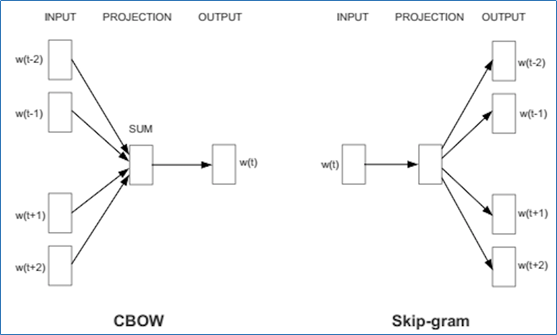
\includegraphics[width=0.85\textwidth]{Figures/Chapter1/word2vec_diagram.png}
  \caption{Architecture of the word2vec model}
  \label{fig:word2vec}
\end{figure}

GloVe authors showed that the ratio of two words' co-occurrence probability (rather than their co-occurrence probabilities themselves) is what conveys information, and that this information is encoded as vector differences. GloVe acquired a lot of traction since they seemed to consistently and significantly outperform standard Distributional Semantic Models. GloVe embedding, however, does not deal well with the problem of polysemy, where the same word has different semantics in different context. This limitation inspires the creation of contextual embedding, with the introduction of transformer models in 2018. Introduced by Vaswani et al in the groundbreaking "Attention is All You Need" paper \cite{DBLP:journals/corr/VaswaniSPUJGKP17}, the Bidirectional Encoder Representations from Transformers (BERT) is a language model that produce tokens which are hugely useful across many NLP tasks. It is distinguished from previous language models by the fact that its learnt representations include context from both sides of the sentences from the architecture that is shown in Figure \fref{fig:bert} below. 

\begin{figure}[htbp]
  \centering
    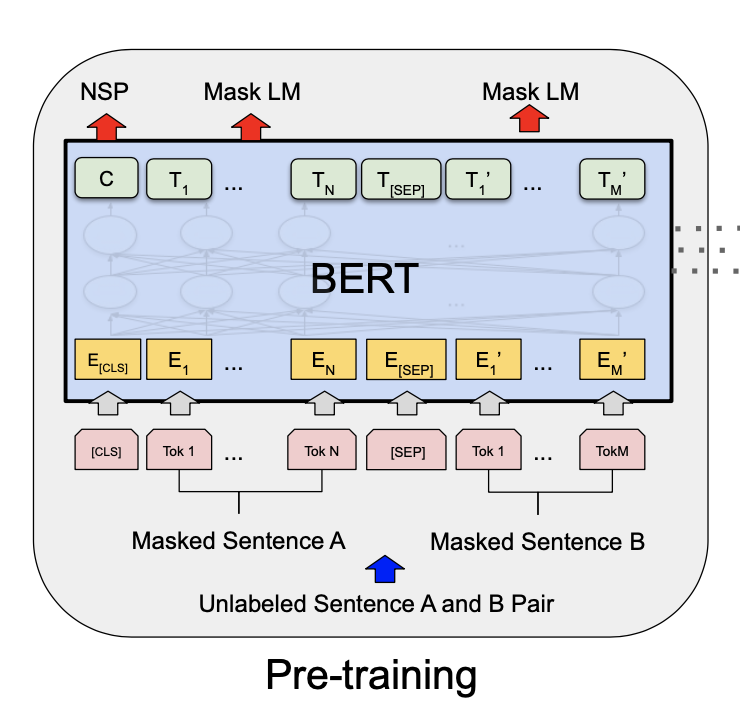
\includegraphics[width=0.85\textwidth]{Figures/Chapter1/bert.png}
  \caption{Bert Architecture}
  \label{fig:bert}
\end{figure}

%introduce the problem of OOV

Despite the major advancement in word embedding research over the last decade, dealing with unknown words still remains as one of the most challenging problems for research and production NLP system. Every NLP model is limited by a fixed-size vocabulary and hence limit the amount of meanings the model can encapsulate about the world. GloVe has a vocabulary size of 40 000 words, and treat any unknown words as OOV while BERT boasts a vocabulary of 30 000 tokens that make uses of sub-words and characters to make sense of an unknown word. As both system are trained on huge corpus of data using tremendous computational power, it is inefficient to retrain the embedding to incorporate new words as NLP systems adapt to the ever-changing environment that they have to operate in. Therefore, in this thesis, we propose a simple method to synthesize a reasonable embedding for a given unknown word. The system is designed to assist mainly in production system, where domain-specific and new words are rare in training corpus but common in production due to high usage from users. An overview of the system supported by this thesis is shown in Figure \fref{fig:workflow} below. 

\begin{figure}[htbp]
  \centering
    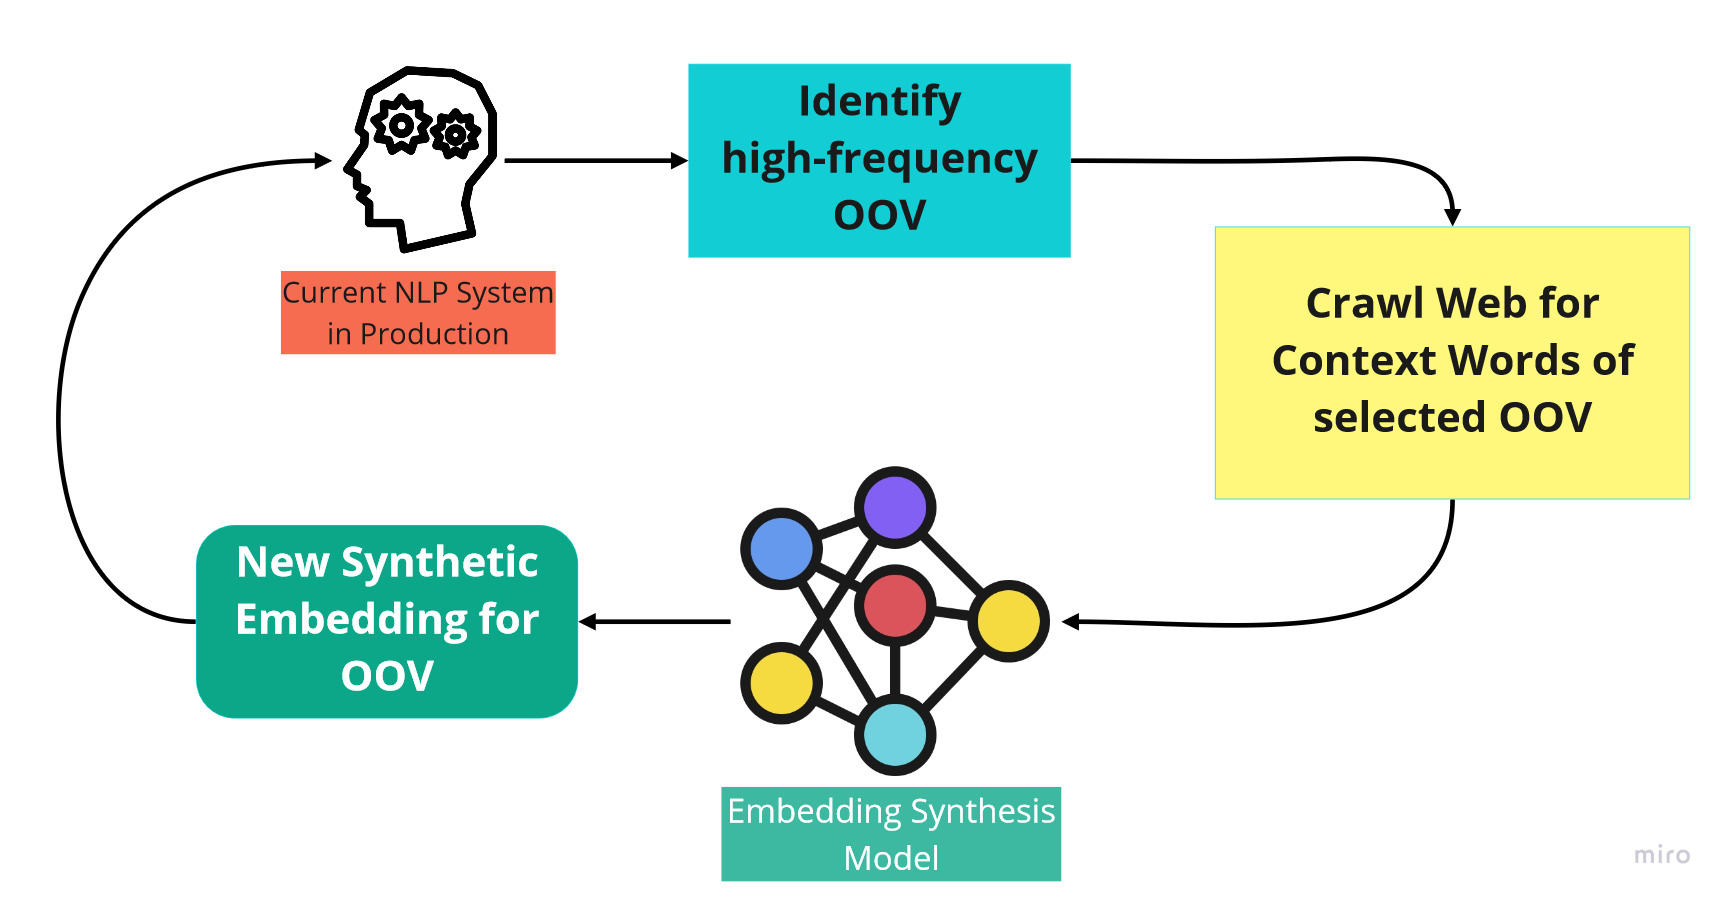
\includegraphics[width=0.85\textwidth]{Figures/Chapter1/workflow.jpg}
  \caption{Workflow of Embedding Synthesis}
  \label{fig:workflow}
\end{figure}

The workflow of the system is as below:

\begin{enumerate}
    \item Current system identify high frequency unknown words that are of high importance
    \item For each word, crawl wiki and related news article about the word 
    \item Pre-process each word and feed it into the embedding synthesis network 
    \item Obtain the new embedding and incorporate it into the current system either via embedding matrix or replacement of embedding
\end{enumerate}

The system is designed to be light-weight and fast to avoid disruption to NLP services in production. The synthetic embedding will help in downstream task to understand unknown words better, with negligible loss. Compared to sub-word segmentation, the synthetic embedding can capture much more semantics information of the word, especially for named entities such as Pfizer. In contrast to pretraining the whole network with OOV corpus, and other sophisticated methods such as ConceptNet ensemble on GloVe \cite{DBLP:journals/corr/VaswaniSPUJGKP17} or Morphology Recurrent Neural Net \cite{luong-etal-2013-better}, the approach in this study is significantly faster and resource-efficient. 

To evaluate the quality of embedding, we follow the suggestion in \cite{schnabel-etal-2015-evaluation}. Relatedness is considered the primary evaluation metric, as analogy is inappropriate in the setting of OOV (which are often rare words). Categorization and Selectional Preference is a feasible metrics but prove to be more challenging to implement. 
% Introduce the 

\newpage

\section{Objectives}

Embedding synthesis is a challenging problem in the research community as there exist no objective metric nor method in creating perfect embedding. Many approaches have been implemented and each of them suffer from their unique limitations, be it resource-heavy or accuracy. In this report, the primary objective is to conduct a study on existing methods and understand their advantages as well as disadvantages. From these understanding, we can create a proof-of-concept model that benefit from the advantages of existing approaches while mitigate as many of the pitfalls as possible. 

The aims of this report are:

\begin{enumerate}
	 \item Design a neural network architecture that are light-weight and is capable of synthesize word embedding
	\item Conduct experiments with different data and hyper-parameters choices on the architecture 
	\item Generate synthetic embedding for a subset of unknown words for GloVe and RoBerta and evaluate these embedding
	\item Provide a method to incorporate existing embedding into system that use GloVe embedding
\end{enumerate}

By securing the above objectives, we will be able to effectively synthesize high-quality embedding in a semi-autonomous manner, thereby greatly reducing the cost and need to retrain the entire network to incorporate meanings of unknown words. As many downstream NLP application such as QA-chatbots and NER suffer from a lack of understanding of unknown words, especially domain-specific named entities, the approach presented in this report can assist NLP engine in production environment by enhancing their capabilities in understanding the text data presented to them by users. 


\newpage

\section{Scope and Assumptions}

The scope of the synthetic embedding generated by the approach in this report is limited to unknown nouns (for training) and named entities of special interest to production such as Pfizer and COVID-19 (for testing). All the related process and methods are developed and tested on online news related to selected keywords. However, it is possible to re-implement the discussed approach in this study, with minor modifications, to adapt it to other unknown words as well. 

The assumptions of the report are:

\begin{enumerate}
    \item Unknown words in NLP production system are typically nouns as they reflect the new trends and phenomena around the world, or cater to services and knowledge in a specific domain. An example of such trend is COVID-19, which has affected many ASR and QA system that are not trained on these words before. Therefore, having a good quality understanding of these words are of special interest as they have potential in enhancing business and services alike. 
    \item The system is designed to trade accuracy and quality reasonably in exchange for a light-weight and fast synthesis method. Cycle time is one of the most crucial factor in user-facing NLP systems, therefore having quick iteration time thanks to fast synthesis can indirectly improve the end-user experience with NLP applications significantly. Additionally, as embedding is used as an input to downstream tasks, a slight reduction in accuracy is acceptable for well-tuned system as they are able to make maximum use of the information captured inside the embedding. 
\end{enumerate}

\newpage

\section{Report Organization}

This report is sectioned into five chapters as follow:
\begin{itemize}
    \item Chapter 1 presents a brief introduction into the project and its background, followed by the project's objectives, scope and assumptions
    \item Chapter 2 focuses on the literature review of existing approaches to synthesize word embedding, followed by a brief discussion on metrics suited for the objective and inspiration to the current approach
    \item Chapter 3 proposes the system design, the methodology and specifications of the system
    \item Chapter 4 details the implementation of each individual component of the system, from data curation and ingestion to output
    \item Chapter 5 presents the experiments results and evaluate its efficacy 
    \item Chapter 6 explores briefly different properties of the synthetic embedding that are useful for production, and gives several recommendations to modifying existing approach
    \item Chapter 7 gives a conclusion to the report and explore possible future work
\end{itemize}

